\documentclass[de]{./../../common/SurferDesc}%%%%%%%%%%%%%%%%%%%%%%%%%%%%%%%%%%%%%%%%%%%%%%%%%%%%%%%%%%%%%%%%%%%%%%%
%
% The document starts here:
%
\begin{document}
\footnotesize
% Weltrekordfl�chen

%%% 1.Tafel

%%%%%%%%%%%%%%%%%%%%%%%%%%%%%


\begin{surferPage}
  \begin{surferTitle}Eine 7-Eck-symmetrische Septik\end{surferTitle}   \\
  Diese einem Weihnachtsstern �hnelnde Fl�che ist vom Grad $7$.  
    Bis vor Kurzem stellte sie noch die maximal bekannte Anzahl, $84$, von reellen
    Singularit�ten auf einer Septik dar;
    erst 2004 hat Oliver Labs diesen Weltrekord auf $99$ verbessert. 

    Die jeweils drei Kissen, die bei der $7$-Eck-symmetrischen Septik (gro�es
    Bild) 
    �bereinander liegen, kommen wie bei der 
    Chmutov Oktik (vorige Fl�che) von der Verwendung der Tchebychev Polynome.
    Daher wundert es nicht, dass auch diese Fl�che eine Variante von
    Chmutovs Fl�chen ist. 
    Hier wurde die ebene Kurve $T_d(x)+T_d(y)$
    durch ein regelm��iges $7$-Eck $S_7(x,y)$ ersetzt:
    \[S_7(x,y) + \lambda \cdot T_d(z) = 0,\]
    f�r ein geeignetes $\lambda\in\RR$. 
    \vspace*{-0.3em}
    \begin{center}
      \begin{tabular}{c@{\qquad}c}
        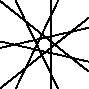
\includegraphics[height=1.5cm]{./../../common/images/labsseptic1.pdf}
        &
        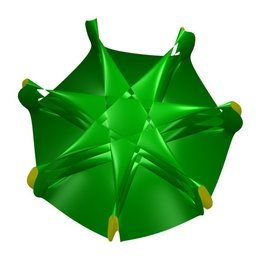
\includegraphics[height=1.5cm]{./../../common/images/septic_7eck_von_oben}
      \end{tabular}
    \end{center}
    \vspace*{-0.3em}    
   Diese Variante von Chmutovs Konstruktion stammt von Duco van
    Straten. 


  \begin{surferText}
     \end{surferText}
\end{surferPage}



\end{document}
%
% end of the document.
%
%%%%%%%%%%%%%%%%%%%%%%%%%%%%%%%%%%%%%%%%%%%%%%%%%%%%%%%%%%%%%%%%%%%%%%%
